\chapter{The MPEG-2 Motion Picture Compression Standard}
\label{chapter:mpeg2}

MPEG-2~\cite{MPEG2} is a popular coding standard for
digital video. 
The scheme is a subset of both the DVD-Video~\cite{Taylor:1999:SDV} 
standard for storing movies, and the Digital Video Broadcasting 
specifications for transmitting HDTV and SDTV~\cite{DVB}. The scheme is
used by a wide variety of multimedia applications and appliances such
as the Tivo Digital Video Recorder~\cite{tivo}, and the DirecTV satellite broadcast
service~\cite{directv}. 

The amount of compression possible depends on the video data. 
Common compression ratios range
from 10:1 to 100:1. For example, HDTV, with a resolution of 1280x720
pixels and a streaming rate of 59.94 frames per second, has an
uncompressed data rate of 1.33 gigabits per second. It is compressed at
an average rate of 66:1, reducing the required streaming rate to
20 megabits per second~\cite{imagevidstandards}.

\begin{figure}
  \begin{center}
    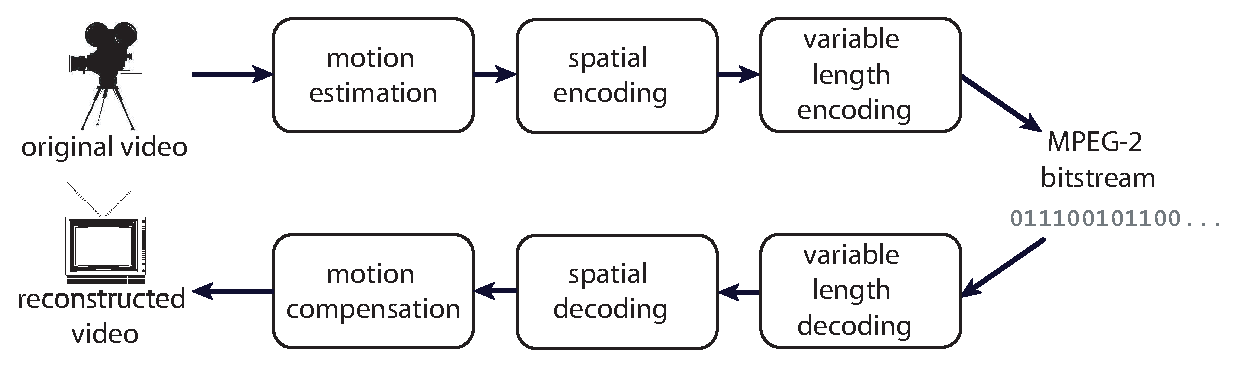
\includegraphics[scale=0.7, angle=0]{./mpeg2_overview.eps}
    \caption{High level view of MPEG-2 decoding and encoding.}
    \label{fig:mpeg2_overview}
  \end{center}
\end{figure}

The MPEG-2 specification contains three types of compression:
variable length coding, spatial coding, and motion prediction.
Figure~\ref{fig:mpeg2_overview} shows a high level overview
of the decoding and encoding process. 
For a complete description of the MPEG-2 data format and coding
scheme one should refer to
the official MPEG-2 standard~\cite{MPEG2}. However, this chapter
contains an abbreviated explanation of the 
standard targeted to a reader lacking prior knowledge of image or video
compression algorithms. The explanation focusses on the 
variable length coding in the parser, 
the functionality needed for spatial coding and decoding,
and the motion prediction components. Iwata et al. estimate that each of these three 
components constitutes a roughly equal portion of the work needed for 
decoding~\cite{iwata98coarse}. Encoding is similar, although
motion estimation constitutes a larger computational effort than
the decoder's motion compensation.

This chapter begins with an enumeration 
of the compression types found in MPEG-2.
It then describes picture organization and the temporal and spatial
transformations that provide compression. 
This is followed by a description of video
organization and finally a list of optional MPEG-2 format extensions.

\section{Compression Techniques}
MPEG-2 uses both {\it lossy} and {\it lossless} compression. 
Lossless compression eliminates redundant information from a signal while allowing
for an exact reconstruction. 
Lossy compression permanently eliminates information from a picture based on
a human perception model. Lossy compression removes details that a casual
observer is likely to miss. A lossy compression is irreversible,
and a lossy decompression process only approximately reconstructs the original
signal. MPEG-2 uses the following compression techniques:

\begin{itemize}
  \item \textbf{Huffman Compression} (\textit{lossless}) 
Huffman compression~\cite{Huffman52} is a form of entropy 
coding. It compresses a signal using variable length codes to efficiently 
represent commonly occurring subpatterns in the signal.
  \item \textbf{Color Channel Downsampling} (\textit{lossy})  
Humans are much better at discerning changes in {\it luminance}, 
than changes in {\it chrominance}. Luminance, or brightness, is a 
measure of color intensity. Chrominance is a measure of color hue.
Pictures are separated into one luminance and two chrominance channels, 
called the \textit{YCbCr} color space. The chrominance channels are
typically downsampled horizontally and vertically. 
  \item \textbf{Frequency Quantization} (\textit{lossy}) 
An image can be expressed as a linear combination of 
horizontal and vertical frequencies.
Humans are much more sensitive
to low frequency image components, such as a blue sky, than to high frequency image components,
such as a plaid shirt. Unless a high frequency component has 
a strong presence in an image, it can be discarded.
Frequencies which must be coded are stored 
approximately (by rounding) rather
than encoded precisely. This approximation process is called
\textbf{quantization}. How the different horizontal and vertical
frequencies are quantized is determined by empirical data
on human perception.
  \item \textbf{Motion Prediction} (\textit{lossless}) 
Frames of a video
contain a great deal of temporal redundancy because much of a
scene is duplicated between sequential frames. Motion estimation is used to
produce motion predictions with respect to one or more reference frames.
Predictions indicate what any given frame should look like. For similar frames, 
only the motion estimate and any error between the predicted values and the
actual values must be encoded.
  \item \textbf{Difference Coding} (\textit{lossless})  
Over any given region in an image the average color value is likely to be
similar or identical to the average color in surrounding regions.
Thus the average colors of regions are coded differentially with respect
to their neighbors. Motion information at neighboring regions is also likely
to be similar or identical and is therefore coded 
differentially with respect to motion at neighboring regions.
\end{itemize}

\section{Picture Organization} 
\label{section:picture_decomp}

\begin{figure}
  \begin{center}
    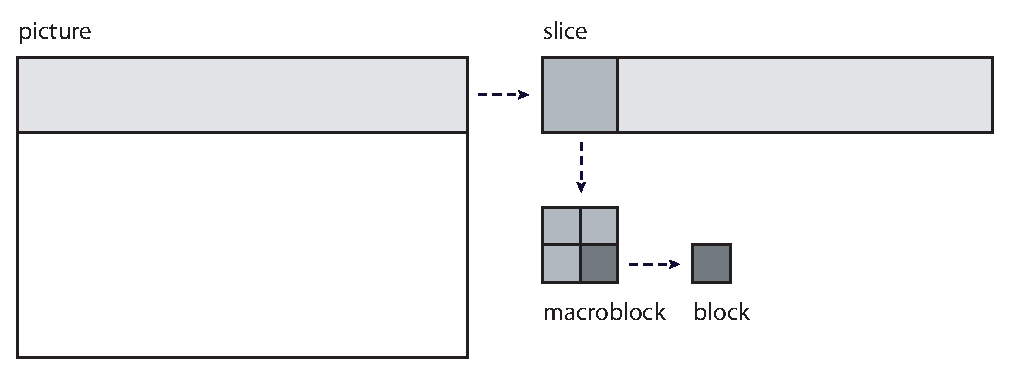
\includegraphics[scale=0.8, angle=0]{./picture_structure.eps}
    \caption{MPEG-2 picture subcomposition.}
    \label{fig:picture_structure}
  \end{center}
\end{figure}

Figure~\ref{fig:picture_structure} shows how the MPEG-2 standard
organizes pictures. Each picture breaks into 
16x16 groups of pixels called \textbf{macroblocks}. 
Adjacent sequences of macroblocks
are contained in a structure called a \textbf{slice}.
Pictures and macroblocks are defined in the
YCbCr color space, and the first step of encoding is
converting the picture into this color representation.

A macroblock is itself composed of 8x8 subpixel 
\textbf{blocks}. There are always
exactly 4 luminance blocks that form a 2x2 array to cover the
macroblock. Because of human insensitivity to chrominance information, each of the two
chrominance channels may be downsampled. 

The type of downsampling in an MPEG-2 stream is called its
\textbf{chroma format}. The two most common chroma formats
are shown in Figure~\ref{fig:chroma_format}. The more common of the two 
is the 4:2:0 format.
This format specifies that each chrominance channel in a macroblock be represented
by a single block, horizontally and vertically
downsampling a macroblock from 16x16 to 8x8 subpixels. 
A 4:2:0 macroblock therefore contains a total of 6 blocks.
An alternate format is 4:2:2. 
The 4:2:2 format uses two blocks for each chrominance 
channel, horizontally downsampling each macroblock from 16x16 to 
8x16 subpixels. 
A 4:2:2 macroblock therefore contains a total of 8 blocks.
A 4:4:4 chroma format also exists but is not commonly used, and specifies 
no color channel downsampling, and uses 4 blocks to 
represent each color channel in a macroblock. 

\begin{figure}
  \begin{center}
    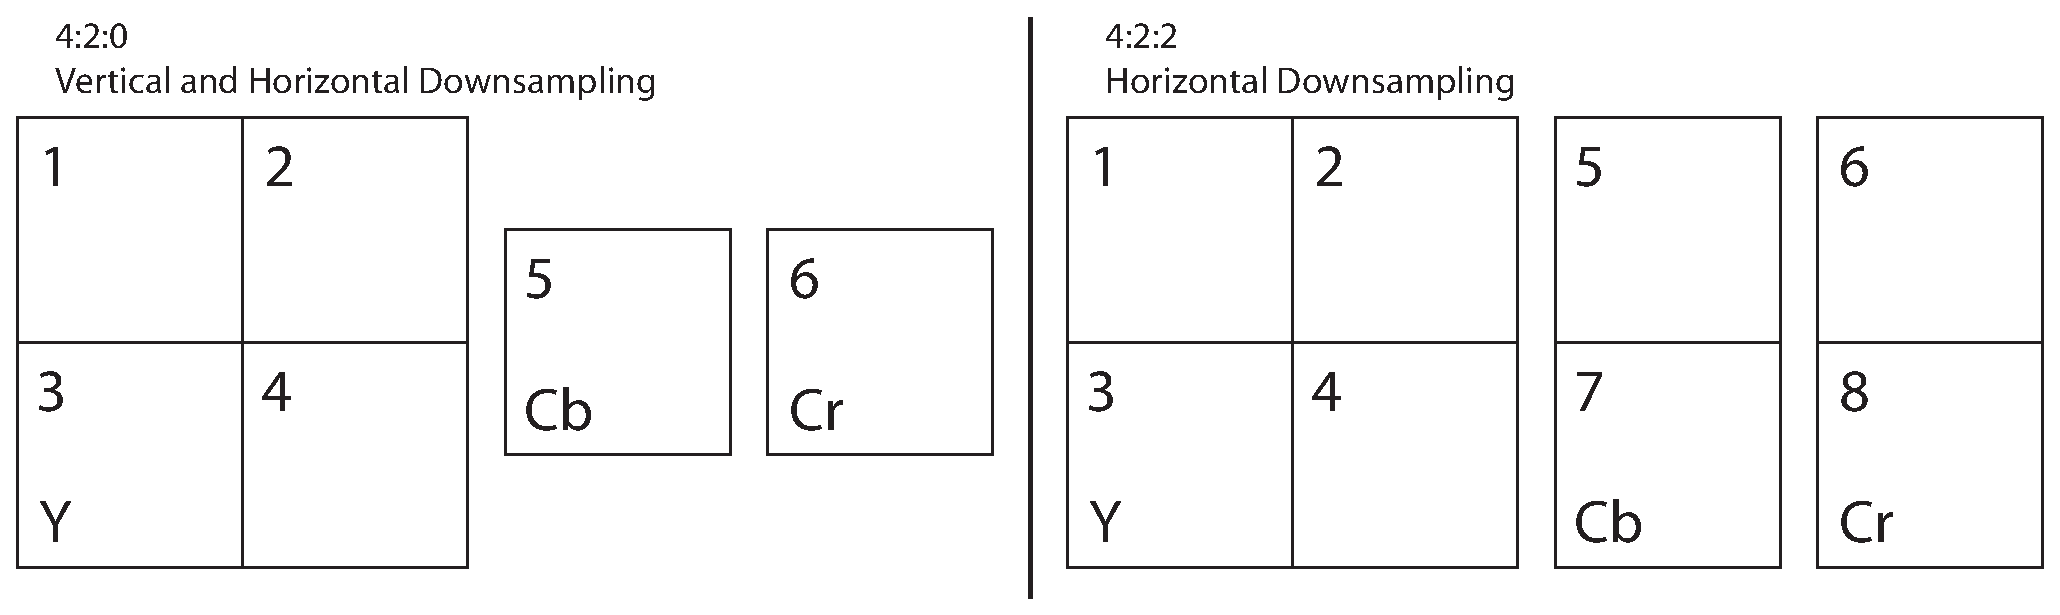
\includegraphics[scale=0.4, angle=0]{./chroma_formats.eps}
    \caption{Commonly used chroma formats.}
    \label{fig:chroma_format}
  \end{center}
\end{figure}

\section{Temporal Compression}

Temporal compression in MPEG-2 is achieved via motion prediction,
which detects and eliminates similarities between macroblocks across
pictures. For any given macroblock $M$, a motion estimator forms a prediction: a \textbf{motion
vector} that contains the horizontal and vertical displacement of that 
macroblock from the most similar macroblock-sized area in one or more reference pictures.
The matching macroblock
is removed (subtracted) from $M$ on a pixel by pixel
basis. The
result is a residual \textbf{predictive coded (P)} macroblock. The residual 
macroblock contains the difference between the motion predicted values for
the macroblock and the macroblock's actual values. A P macroblock
always uses forward motion prediction, meaning that the reference frame
precedes it temporally. (See Section~\ref{subsection:pic_org} for more details on
picture referencing and organization.) Figure~\ref{fig:motion_estimation_forward} illustrates
forward motion estimation.

\begin{figure}[h]
  \begin{center}
    \includegraphics[scale=0.5, angle=0]{./motion_estimation_forward_vectorized.eps}
    \caption{Eliminating temporal redundancy through forward motion estimation.}
    \label{fig:motion_estimation_forward}
  \end{center}
\end{figure}

Macroblocks encoded without the use of motion
prediction are \textbf{intra coded (I)} macroblocks. 
In addition to the forward motion 
prediction used by P macroblocks, it is possible to 
encode new macroblocks using motion
estimation from both temporally previous and subsequent pictures. Such macroblocks
are \textbf{bidirectionally predictive coded (B)} macroblocks, and they exploit a
greater amount of temporal locality. A B macroblock may contain two motion vectors, 
referencing both previous and subsequent pictures; in this case, the 
motion prediction
is an unweighted average of the forward and backward predictions. 
Figure~\ref{fig:motion_estimation_back}
illustrates backward motion estimation.

\begin{figure}[h]
  \begin{center}
    \includegraphics[scale=0.5, angle=0]{./motion_estimation_back_vectorized.eps}
    \caption{Eliminating temporal redundancy through backward motion estimation.}
    \label{fig:motion_estimation_back}
  \end{center}
\end{figure}

All blocks in macroblocks, whether intra coded or residually encoded, undergo 
spatial compression.
Except for the first macroblock in a slice, 
motion vectors are compressed by coding them differentially with respect to the 
motion vectors in the previously decoded 
macroblock\footnote{A second exception is for the first set of
motion vectors following an intra coded macroblock. These vectors 
must always be fully coded because intra coded macroblocks have no motion
vectors.}.

\section{Spatial Compression}
\label{sec:MPEGspatial}

Each block undergoes a two-dimensional \textbf{Discrete Cosine Transform} (DCT),
which is a frequency transform that separates the block into components
with varying visual importance. As shown in Figure~\ref{fig:dct}, 
the DCT takes one 8x8 block as input and produces a 
transformed 8x8 block of frequency coefficients as output. 
Horizontal frequency increases towards the right of the block and
vertical frequency increases towards the bottom of the block.
The upper left corner of the block contains the lowest frequencies
and the lower right corner contains the highest frequencies.

\begin{figure}
  \begin{center}
    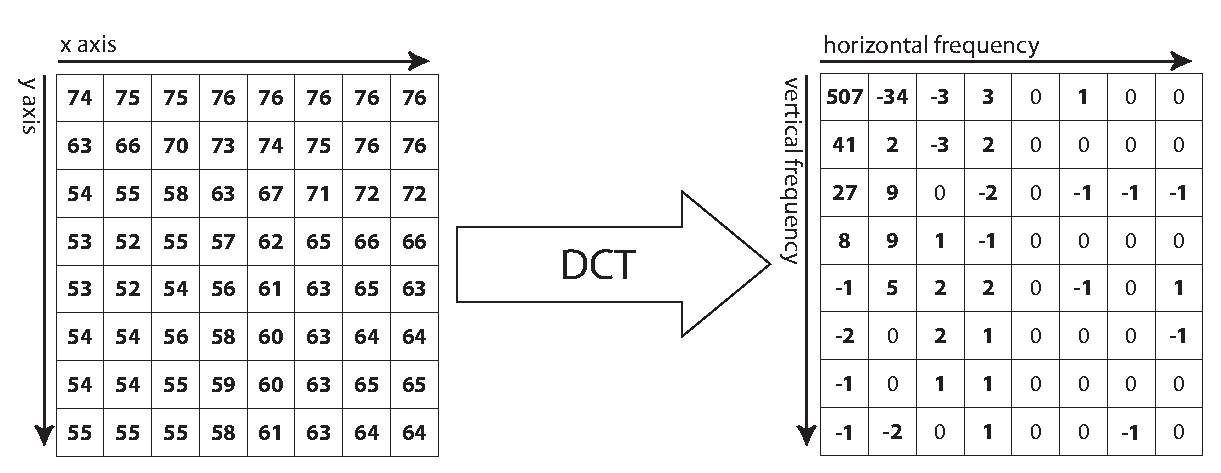
\includegraphics[scale=0.6, angle=0]{./dct.eps}
    \caption{Sample input and output for a discrete cosine transform.}
    \label{fig:dct}
  \end{center}
\end{figure}

The DCT by itself is lossless\footnote{I ignore a possible loss of 
precision, an issue addressed by the MPEG-2 specification and explained
subsequently in Section~\ref{subsection:extra_decoder}}
but enables the quantization of blocks according to a 
\textbf{quantization table} of \textbf{quantization values}, 
also in the frequency domain. The quantization table reflects
a human's relative abilities to discern different frequency
components of an image. 
The quantization table itself may contain any values and can be
specified in the MPEG-2 bitstream, although usually one 
of several standard tables is used.
Each value in a frequency-transformed
block is divided by the corresponding quantization value, with
any remainder thrown away. An example block quantization appears
in Figure~\ref{fig:quantize}\footnote{The quantization process is
technically more complicated than the math I have just described,
although the description is conceptually accurate. The output block
in the figure is accurately quantized, but cannot be arrived at by
the division process I just described.}.
A small error may be introduced
to individual frequency components and most low energy frequency components
are simply reduced to $0$. This stage introduces much of the lossy 
compression in MPEG-2 coding. 

\begin{figure}[h]
  \begin{center}
    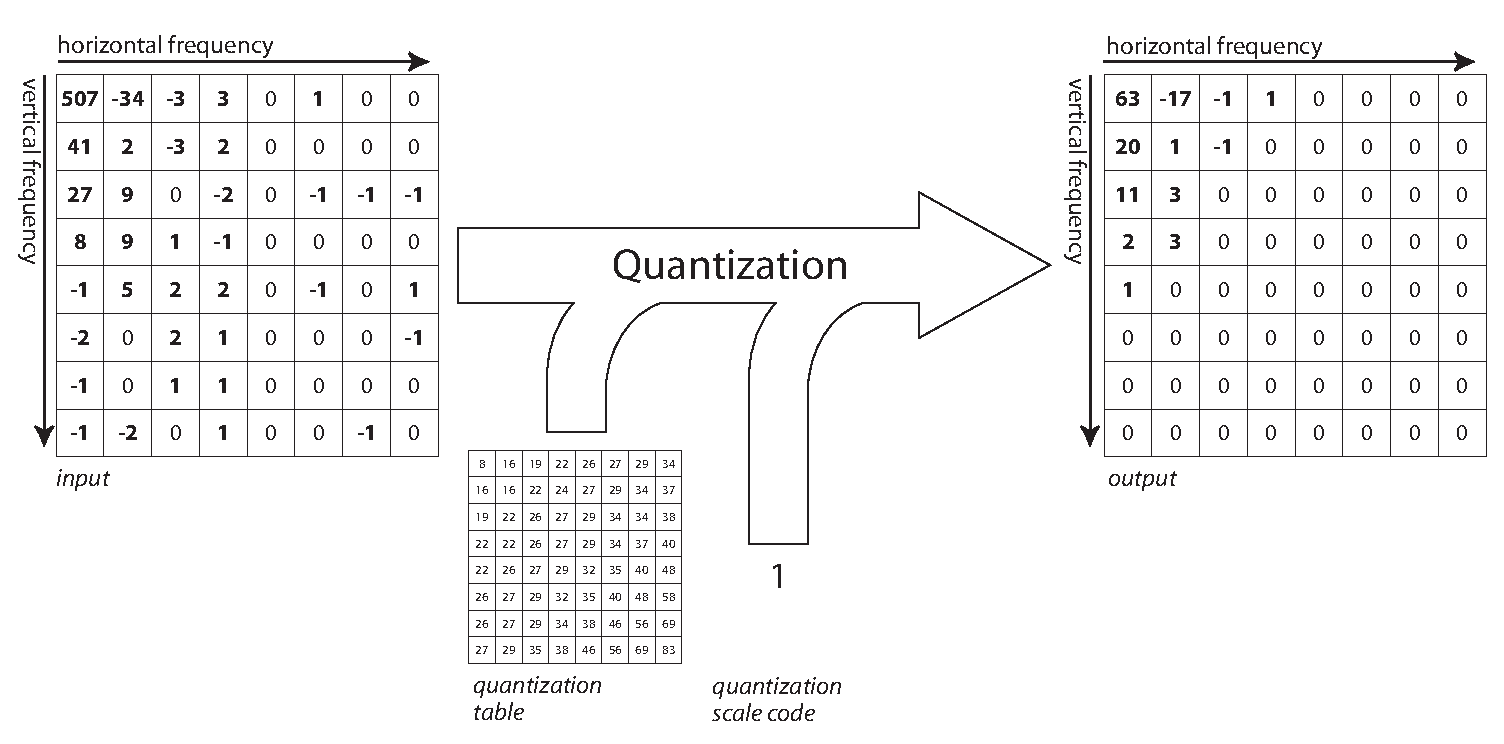
\includegraphics[scale=0.6, angle=0]{./quantization_example2.eps}
    \caption{Example block quantization.}
    \label{fig:quantize}
  \end{center}
\end{figure}

MPEG-2 uses two quantization tables. One table is used for all 
intra coded blocks and the other for residually coded blocks. 
At irregular intervals, an MPEG-2 bitstream indicates a 
\textbf{quantization scale code} which provides an additional 
scaling factor that affects all frequencies in a block. 
One can adjust the desired compression level and
control the video bitrate (bits per second)
by tuning the quantization scale code between macroblocks. 
In an encoder this control 
is typically realized using feedback about the final entropy coded 
output bitrate earlier in the quantization stage.

The upper left value in the frequency transformed block contains the
\textbf{DC coefficient}, which
is the coefficient corresponding to the zero frequency
in both the horizontal and vertical dimensions. Less formally,
this is the average color of the block. 
MPEG-2 differentially encodes the DC block value for 
intra coded blocks. 
The first DC coefficient in the first block in a slice is fully
encoded and all subsequent DC coefficients in a slice are 
differentially coded. Note that the differential coding
semantics for DC coefficients and motion vectors guarantee that
macroblocks in different slices are coded
independently from each other.

After quantization a block is \textbf{zigzag} ordered. 
Zigzag ordering sorts a
block's values from lowest to highest frequency. Since
low-frequency components are more likely to have non-zero 
values following quantization, zigzag ordering consolidates 
non-zero block coefficients together at the beginning of the block. 
The zigzag order commonly used by MPEG-2 is shown in Figure~\ref{fig:zigzag_order}

\begin{figure}
  \begin{center}
    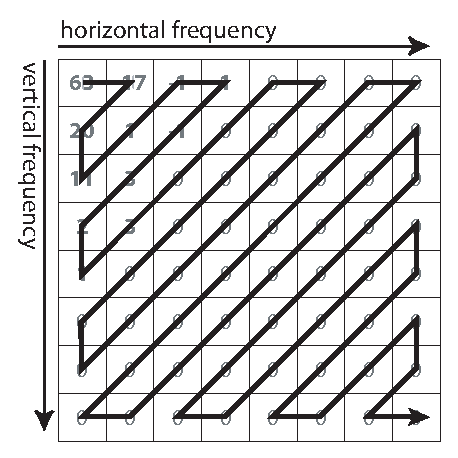
\includegraphics[scale=0.6, angle=0]{./zigzag_order.eps}
    \caption{Zigzag ordering of frequency coefficients from low to high.}
    \label{fig:zigzag_order}
  \end{center}
\end{figure}

The zigzag ordered data is then Huffman compressed using 
a set of predefined Huffman tables defined in the MPEG-2 
specification. Picture metadata, such as the picture type, changes
to the quantization scale code, and motion vectors,
are also Huffman encoded and interleaved in the bitstream.

\section{Required Block Decoding Components}
\label{subsection:extra_decoder}

Data transformation pairs such as a DCT and an inverse DCT (IDCT), may accidentally
introduce loss of data precision, 
due to hardware architecture and algorithm differences 
in a decoder and encoder.
While such imprecisions are tiny, the use of temporal compression
means that small imprecisions accumulate and magnify over the course
of several motion predicted pictures and quickly become noticeable.
For this reason the MPEG-2 specification places specific functional constraints on
mathematical operations in MPEG-2 codecs: 

\begin{itemize}
\item The frequency coefficients emitted from the inverse quantization stage must be saturated within predefined levels.
\item The low-order bit of the highest frequency value in a block is used as a parity bit on the value of the block. In the encoder this bit is set between the DCT and quantization. In the decoder the bit is checked between the saturated inverse quantization and the IDCT. This setting and checking of the bit is called \textbf{mismatch control}.
\item The output of the IDCT is saturated within predefined levels.  
\end{itemize}

\section{Video Organization}

\label{subsection:pic_org}

Just as macroblocks have an associated I, P, or B type, 
pictures also have an associated type, used to 
limit the kinds of macroblocks that they may contain. I pictures 
contain only I macroblocks, P pictures contain I or P macroblocks, 
and B pictures may contain I, P, or B macroblocks. Only I and P 
pictures are used as references for motion prediction and
all I and P pictures are automatically considered references. 
B pictures are never used as references. 

The highest level of organization in an MPEG-2 data stream
is the \textbf{Group of Pictures} (GOP), which 
contains all the information needed to reconstruct a temporally continuous sequence of
video. GOPs consist of I, P, and B pictures.
A typical I:P:B picture ratio in a GOP is 1:3:8, and a typical
picture pattern is a repetition of the following logical sequence,
where the subscripts denote the temporal ordering of the pictures in the video:
\begin{center}
I$_1$~B$_2$~B$_3$~P$_4$~B$_5$~B$_6$~P$_7$~B$_8$~B$_9$~P$_{10}$~B$_{11}$~B$_{12}$~I$_{13}$~$\cdot$~$\cdot$~$\cdot$
\end{center}

Any backwards motion vector in a picture refers to the immediately preceding
reference picture. Likewise, any forward motion vector refers to the subsequent
reference picture. To simplify the decoding process, pictures are not ordered
temporally in the data stream, but rather in the order that they are needed for decoding:
P pictures are always coded with respect to the previous
reference picture and B pictures are always coded with respect to the previous two
reference pictures. Thus, the picture pattern previously described is ordered
in the MPEG-2 data stream as:
\begin{center}
I$_1$~P$_4$~B$_2$~B$_3$~P$_7$~B$_5$~B$_6$~P$_{10}$~B$_8$~B$_9$~I$_{13}$~B$_{11}$~B$_{12}$~$\cdot$~$\cdot$~$\cdot$
\end{center}

\section{Additional MPEG-2 Features}
\label{additional:mpeg}
Because MPEG-2 targets a wide range of devices, the specification is complicated by additional features that make decoding any given video possible on a range of architectures. The following features are mentioned for the sake of completeness, but are excluded from the StreamIt MPEG-2 codec implementations. These features constitute alternative data formats, rather than compression or algorithmic enhancements, and are suitable for exclusion in research-oriented MPEG-2 implementations.

\begin{itemize}
\item \textbf{Interlacing} is a legacy television format needed to support many analog output devices. An interlaced frame contains only half of the original picture data, leaving out alternating horizontal lines. Sequential frames alternate between encoding even and odd scan lines. The alternative to interlacing, which fully encodes each picture, is called \textbf{progressive scan}. 
\item The MPEG-2 bitstream can contain \textbf{layers} which contain alternate encodings of the same picture. A motivating example for this feature is the DVD format, which typically encodes an interlaced version of a movie in the primary layer, and an interlaced version containing the alternate scan lines in a secondary layer. Devices that output interlaced pictures can ignore the secondary layer and devices that output progressive pictures can combine the two layers to produce the complete video.
\item \textbf{Concealment motion vectors} indicate motion estimates for intra-coded macroblocks. These concealment motion vectors are only used to form a macroblock prediction if bitstream errors prevent correct recovery of blocks contained in the macroblock. This plays an important role in the decoding of broadcast MPEG-2 streams such as satellite or HDTV, where transport errors are likely to occur.
\end{itemize}
